\chapter{RESULTADOS OBTIDOS}\label{sec:resultados}
\justifying

%\begin{itemize}
%	\item \textcolor{red}{IGOR: já fiz uma primeira revisão deste capítulo e indico em vermelho o que deve fazer para melhorar este capítulo. Tudo que acrescentar ou mudar coloque em azul.} \textcolor{green}{OK}
%	\item \textcolor{red}{IGOR: não está aparecendo a numeração das Figuras no caption. Algo de errado está acontecendo no modelo que está utilizando.} \textcolor{green}{OK}
%	\item \textcolor{red}{IGOR: está errada a citação do trabalho do método de Duan e Zamir (1995), não é a citação que colocou \cite{Duan}.}\textcolor{green}{\textbf{OK}}
%\end{itemize}

Neste capítulo, resultados obtidos com a ferramenta computacional construída são apresentados.

%--------------------------------------------------------------------------------%
\section{SIMULAÇÕES HEMODINÂMICAS}\label{sec:simulacoes}

 Nesta seção, apresentam-se resultados obtidos atrabés das simulações do modelo matemático de Duan e Zamir~\cite{Duan1992} usando a ferramenta computacional desenvolvida tanto no ambiente InGU quanto no ambiente IGU. As simulações realizadas aqui tratam da propagação de uma onda harmônica simples ao longo de uma árvore, onde reflexões de onda modificam a amplitude da onda de pressão enquanto ela avança. 
 
 A escolha de uma onda harmônica simples neste estudo possibilita investigar os efeitos da frequência, fluido viscoso e viscoelasticidade da parede do segmento de vaso.

Considerou-se também neste estudo um modelo de árvore arterial canina como ilustrado na Figura~\ref{fig:arvore-canina}. As propriedades dos segmentos foram escolhidas oriundas dos dados de Fung~\cite{fung2013biomechanics} e são descritas na Tabela~\ref{tab1:proprerty}. 

\begin{figure}[!htbp]
	\centering
	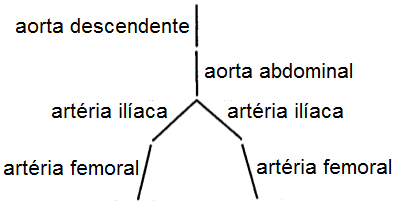
\includegraphics[scale=0.8]{Figures/tree_canine.png}
	\caption{Representação do modelo de árvore arterial canina (figura adaptada de~\cite{Duan}).}
	\label{fig:arvore-canina}
\end{figure}

\begin{table}[!htbp]
	\caption{Propriedades dos vasos do modelo de árvore arterial~\cite{Duan,Fung}}
	\centering{}
	\begin{tabular}{c|c|c|c|c|c}
		\toprule 
		Artéria	& Comprimento & Densidade & Viscosidade  & Diâmetro & Módulo de  \\ 
		& ($cm$) & $\rho$ ($g/cm^3$) & $\mu_0$ ($g/cm s$) & ($cm$) & Young ($dyn/cm^2$) \\ 
		\midrule 
		Aorta & 25 & $0,960$ & 0,0385 & 1,3 &4,8 $\times 10^6$ \\ 
		Descendente &  & &  & & \\ 
		\hline 
		Aorta & 11 & $1,134$ & 0,0449 & 0,9 & 1,0 $\times 10^7$ \\
		Abdominal &  & &  & &  \\ 
		\hline 
		Ilíaca & 12 & $1,172$ & 0,0472 & 0,6 & 1,0 $\times 10^7$\\ 
		\hline 
		Femoral & 10 & $1,235$ & 0,0494 & 0,4 & 1,0 $\times 10^7$\\ 
		\bottomrule 
	\end{tabular} 
	\label{tab1:proprerty}
\end{table}

Nas simulações realizadas, calculou-se a distribuição de amplitude de pressão ao longo da árvore arterial (Figura~\ref{fig:arvore-canina}). Os resultados foram obtidos para quatro diferentes frequên\-cias e três diferentes cenários de escoamento/segmento: (i) escoamento viscoso em segmento puramente elástico (cenário 1 da Seção~\ref{sec:cenario}), (ii) escoamento invíscido em segmento viscoelástico (cenário 2) e (iii) escoamento viscoso em segmento viscoelástico (cenário 3). 

Os resultados obtidos nas simulações são mostrados nas Figuras~\ref{fig3a:arterial-tree}, \ref{fig3b:arterial-tree}, \ref{fig4a:arterial-tree}, \ref{fig4b:arterial-tree}, \ref{fig5a:arterial-tree} envolvendo a amplitude da pressão ao longo do modelo de árvore arterial. Nestas figuras, o comprimento de cada segmento arterial foi dimensionado para $1,0$, de modo que o comprimento adimensional total da árvore é $4,0$. O comprimento real é $58$ cm. A amplitude da pressão também foi escalada pela pressão de entrada $P_o = 1$, e os resultados finais são portanto mostrados em termos de amplitude de pressão adimensional $|P|$ versus a distância adimensional $X$ do início da árvore.


%--------------------------------------------------------------------------------%
\subsection{ESCOAMENTO VISCOSO}\label{sec:cenario1}

Nas Figuras~\ref{fig3a:arterial-tree} e \ref{fig3b:arterial-tree}, o efeito da viscosidade do fluido é examinado separadamente conside\-ran\-do-se o escoamento em vasos puramente elásticos com quatro valores diferentes de viscosidade do fluido, ou seja, $\mu = 0$; $0,5 \mu_0$; $1,0 \mu_0$ e $1,5 \mu_0$, onde $\mu_0$ é o valor base da viscosidade da Tabela~\ref{tab1:proprerty}. Observa-se que o efeito da viscosidade do fluido é reduzir o aumento global na amplitude da onda de pressão causada pelas reflexões das ondas à medida que a onda se desloca na direção à jusante. Além disso, modera os picos locais na distribuição de pressão.

\begin{figure}[!htbp]
	\centering
	(a) \\
	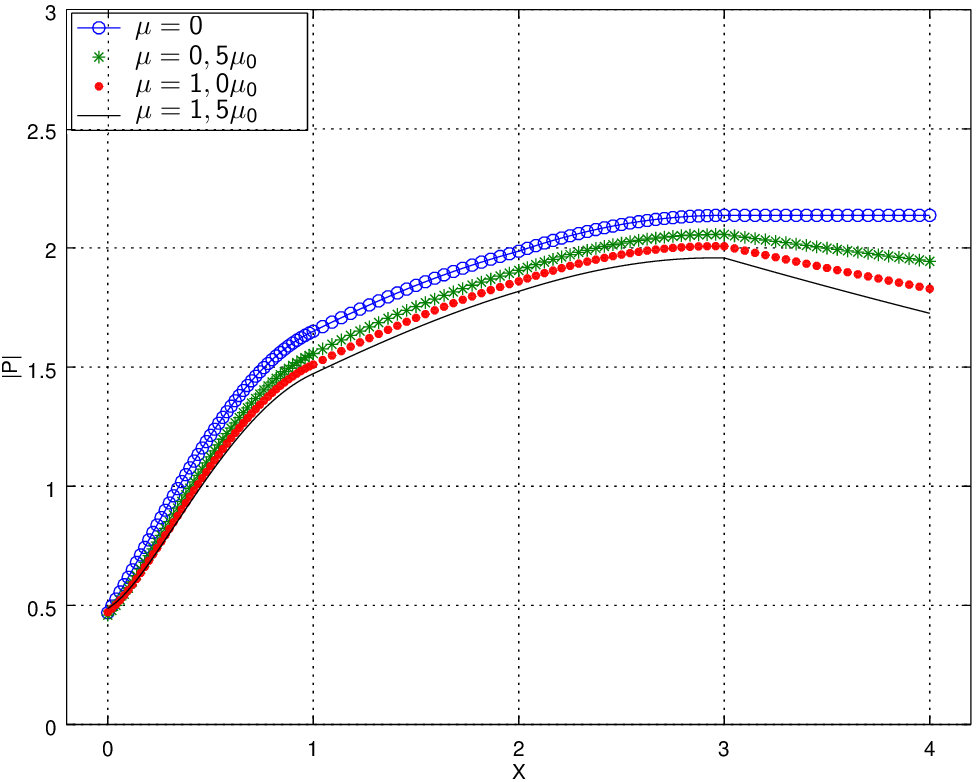
\includegraphics[scale=0.7]{Figures/fig3_P_f3_65_visc_NEW.png}\\
	(b)\\
	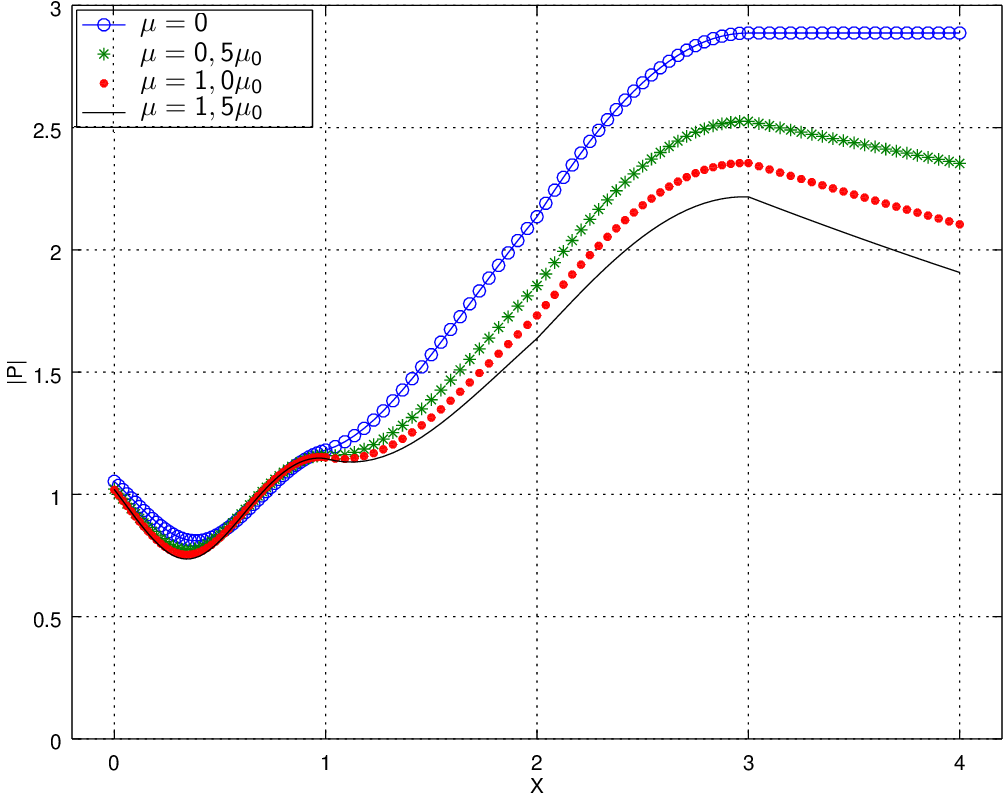
\includegraphics[scale=0.7]{Figures/fig3_P_f7_30_visc_NEW.png}\\
	\caption{Amplitude da pressão $|P|$ ao longo da árvore arterial considerando diferentes viscosidade do fluido $\mu$ e frequências: (a) $f$ = 3,65 Hz, (b)  $f$ = 7,30 Hz. }
	\label{fig3a:arterial-tree}%
\end{figure}

\begin{figure}[!htbp]
	\centering
	(a) $f$ = 10,95 Hz\\
	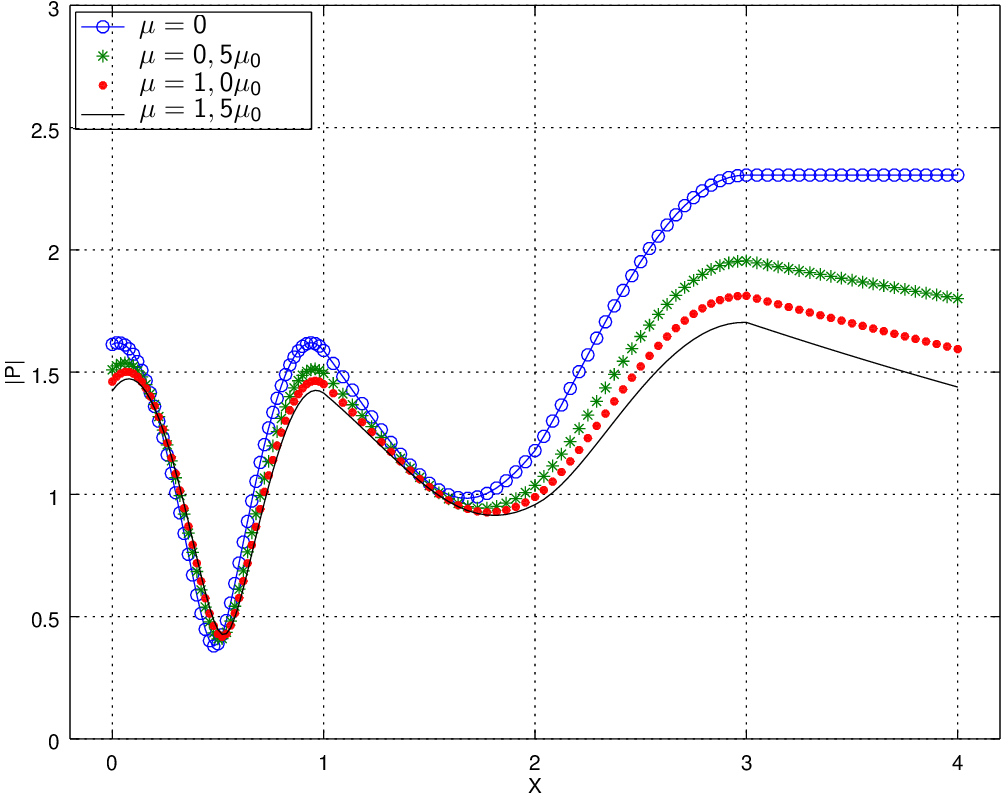
\includegraphics[scale=0.7]{Figures/fig3_P_f10_95_visc_NEW.png}\\
	(b) $f$ = 14,60 Hz\\
	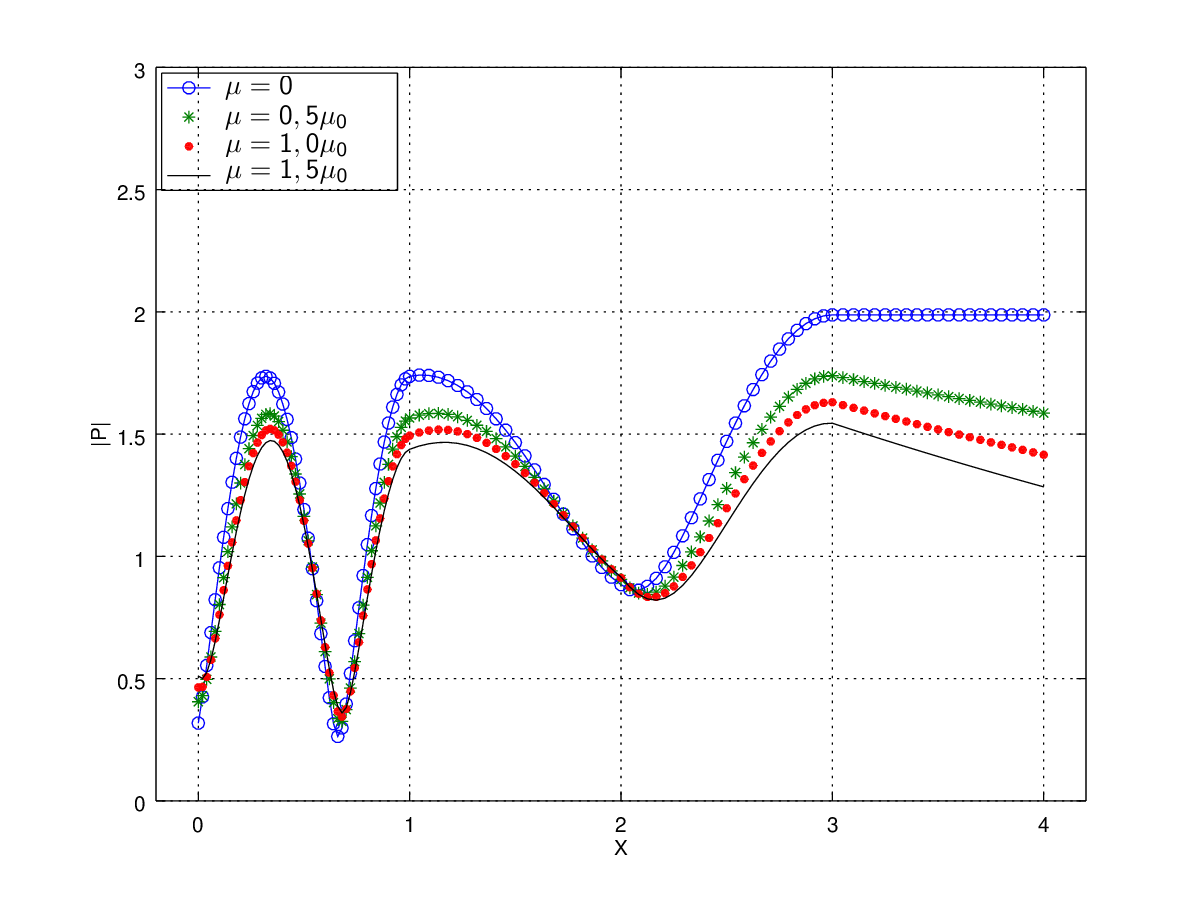
\includegraphics[scale=0.7]{Figures/fig3_P_f14_60_visc_NEW.png}\\
	\caption{Amplitude da pressão $|P|$ ao longo da árvore arterial considerando diferentes viscosidade do fluido $\mu$ e frequências: (a) $f$ = 10,95 Hz, (b)  $f$ = 14,60 Hz. }
	\label{fig3b:arterial-tree}%
\end{figure}

%--------------------------------------------------------------------------------%
\subsection{VASO VISCOELÁSTICO}\label{sec:cenario2}

Nas Figuras~\ref{fig4a:arterial-tree} e \ref{fig4b:arterial-tree}, o efeito da viscoelasticidade da parede do vaso é considerado separadamente considerando-se o escoamento invíscido e tomando-se quatro valores diferentes da viscoelasticidade da parede do vaso. O modelo viscoelástico proposto utilizado para fins destes cálculos é apresentado no cenário 2 da Seção~\ref{sec:cenario}, no qual a viscoelasticidade da parede do vaso é representada por um módulo de Young complexo. Estas figuras mostram os resultados para $\phi_0$ = $0^o$, $4^o$, $8^o$ e $12^o$. Quando $\phi_0$ = $0^o$, tem-se um valor representando uma parede puramente elástica e para $\phi_0> 0$ tem-se a representação da viscoelasticidade. Nota-se a partir destas figuras que o efeito da viscoelasticidade, como o da viscosidade do fluido, é amortecer o aumento global da amplitude da onda de pressão causada pelas reflexões das ondas à medida que a onda se desloca na direção à jusante, bem como moderar os picos locais na distribuição de pressão. 

\begin{figure}[!htbp]
	\centering
	(a) $f$ = 3,65 Hz \\
	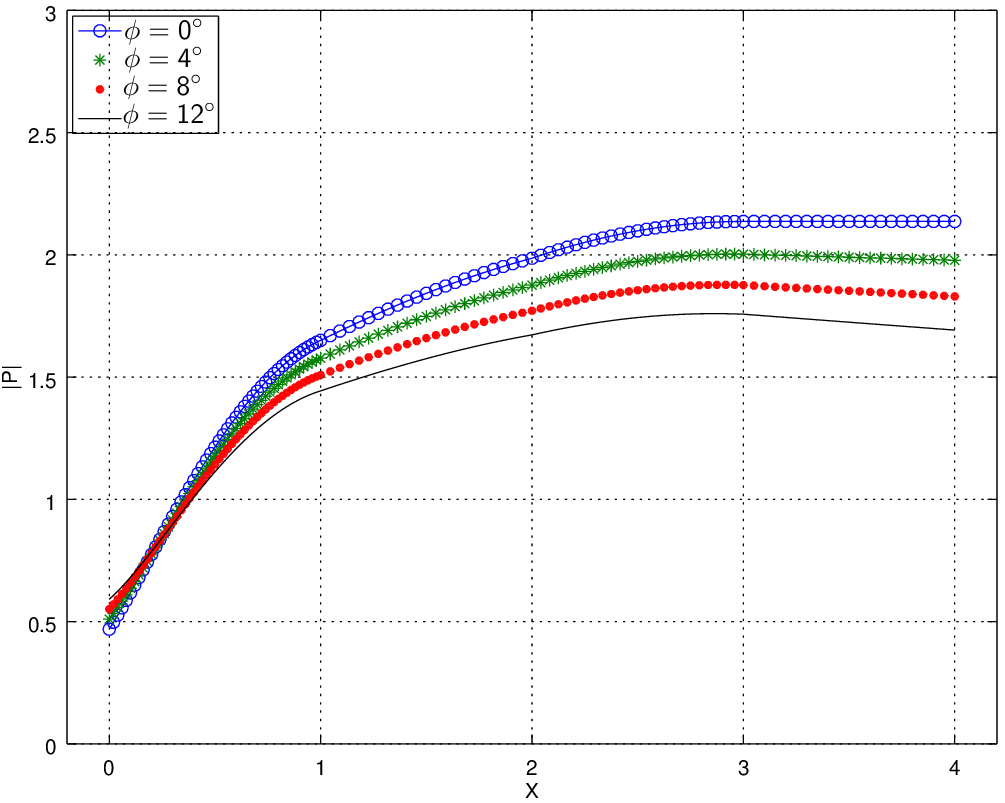
\includegraphics[scale=0.7]{Figures/fig4_P_f3_65_viscoelasticity_NEW.png}\\
	(b)  $f$ = 7,30 Hz\\
	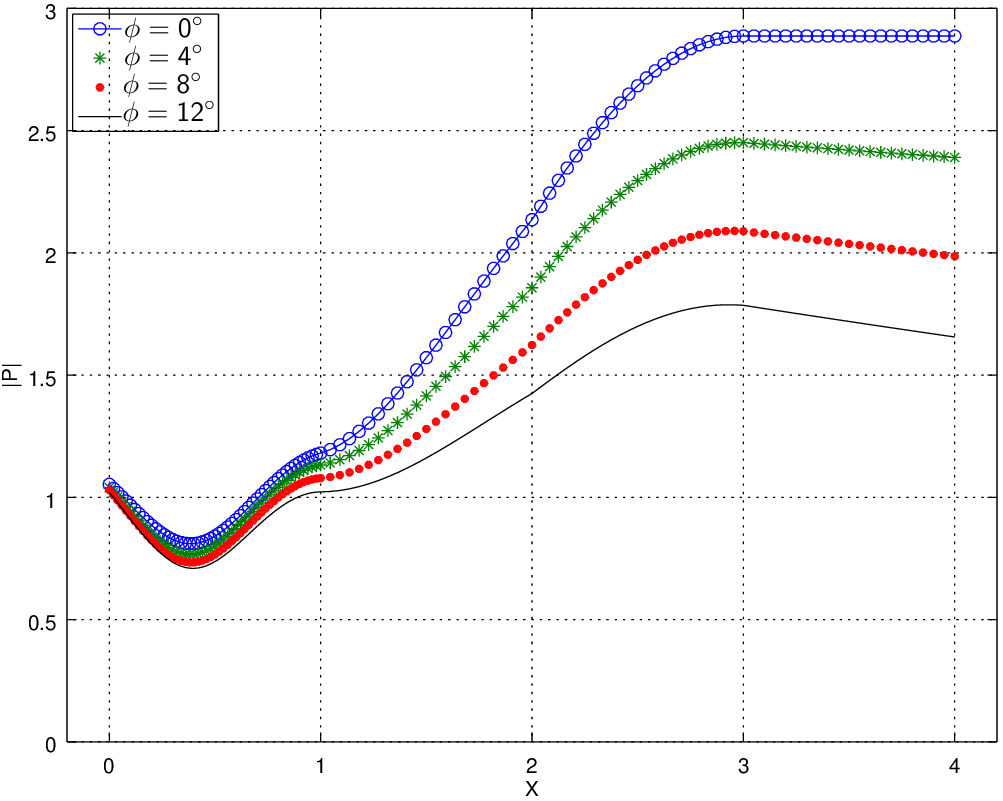
\includegraphics[scale=0.7]{Figures/fig4_P_f7_30_viscoelasticity_NEW.png}\\
	\caption{Amplitude da pressão $|P|$ ao longo da árvore arterial considerando diferentes valores de viscoelasticidade $\phi_0$ e frequências: $f$ = 3,65 Hz e  $f$ = 7,30 Hz. }
	\label{fig4a:arterial-tree}%
\end{figure}

\begin{figure}[!htbp]
	\centering
	(a) $f$ = 10,95 Hz\\
	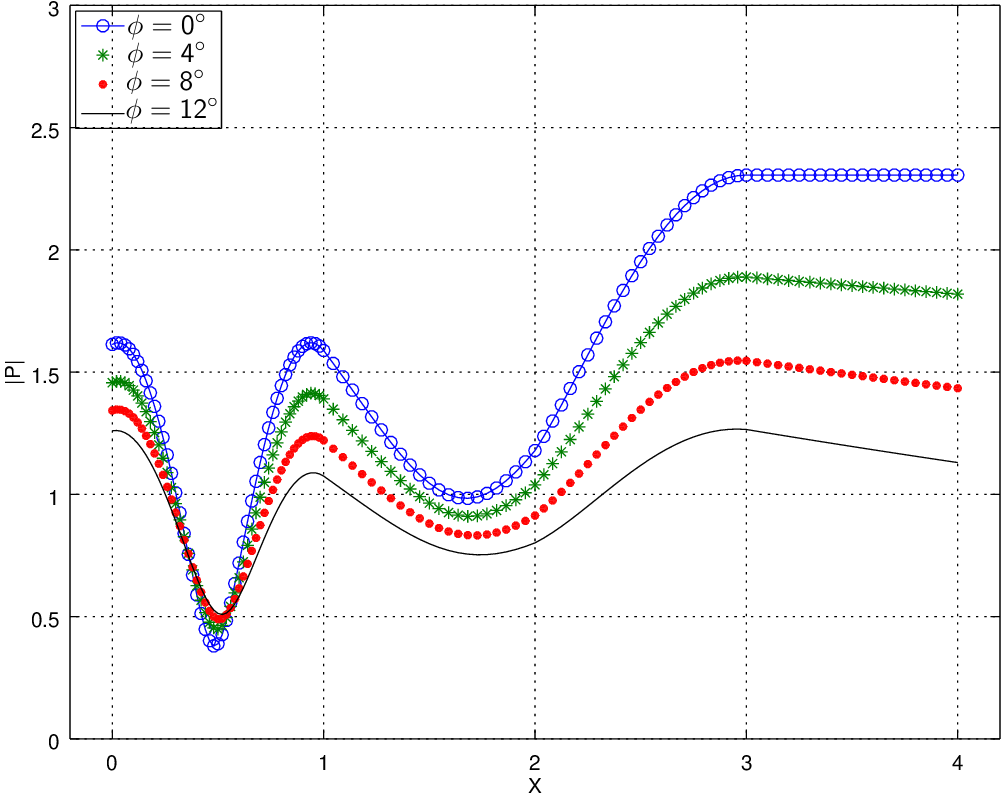
\includegraphics[scale=0.7]{Figures/fig4_P_f10_95_viscoelasticity_NEW.png}\\
	(b) $f$ = 14,60 Hz\\
	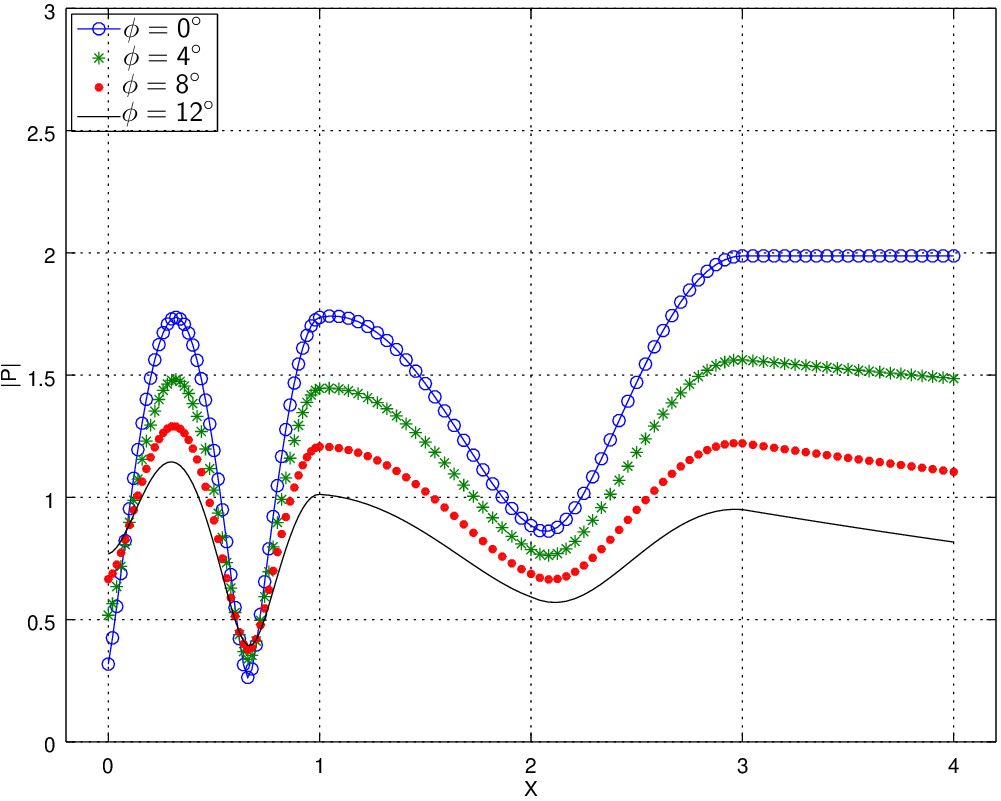
\includegraphics[scale=0.7]{Figures/fig4_P_f14_60_viscoelasticity_NEW.png}\\
	\caption{Amplitude da pressão $|P|$ ao longo da árvore arterial considerando diferentes valores de viscoelasticidade $\phi_0$ e frequências: $f$ = 10,95 Hz e $f$ = 14,60 Hz.}
	\label{fig4b:arterial-tree}%
\end{figure}

%--------------------------------------------------------------------------------%
\subsection{ESCOAMENTO VISCOSO EM VASO VISCOELÁSTICO}\label{sec:cenario3}

Nas Figuras~\ref{fig5a:arterial-tree}, \ref{fig5b:arterial-tree}, o efeito da viscoelasticidade da parede do segmento é adicionada ao efeito do escoamento viscoso, adotando dois valores diferentes da viscoelasticidade e dois valores de viscosidade. O modelo utilizado no cenário 3 é a soma dos efeitos apresentados na Seção~\ref{sec:cenario}, adicionando o fator viscoso e o módulo de Young complexo. Estas figuras mostram o resultado para $\phi_0$ = $0^o$, $8^o$ e com as viscosidades $\mu = 0$ e $0,5 \mu_0$. Ao visualizar os efeitos da viscoelasticidade e viscosidade na amplitude da onda de Pressão $P$, é observado o amortecimento global da amplitude de onda de pressão, somado à moderação dos picos locais na distribuição de pressão. Entretanto, o efeito somado dos fenômenos causa um amortecimento mais eficaz que o visto nos outros cenários.

\begin{figure}[!htbp]
	\centering
	(a) \\
	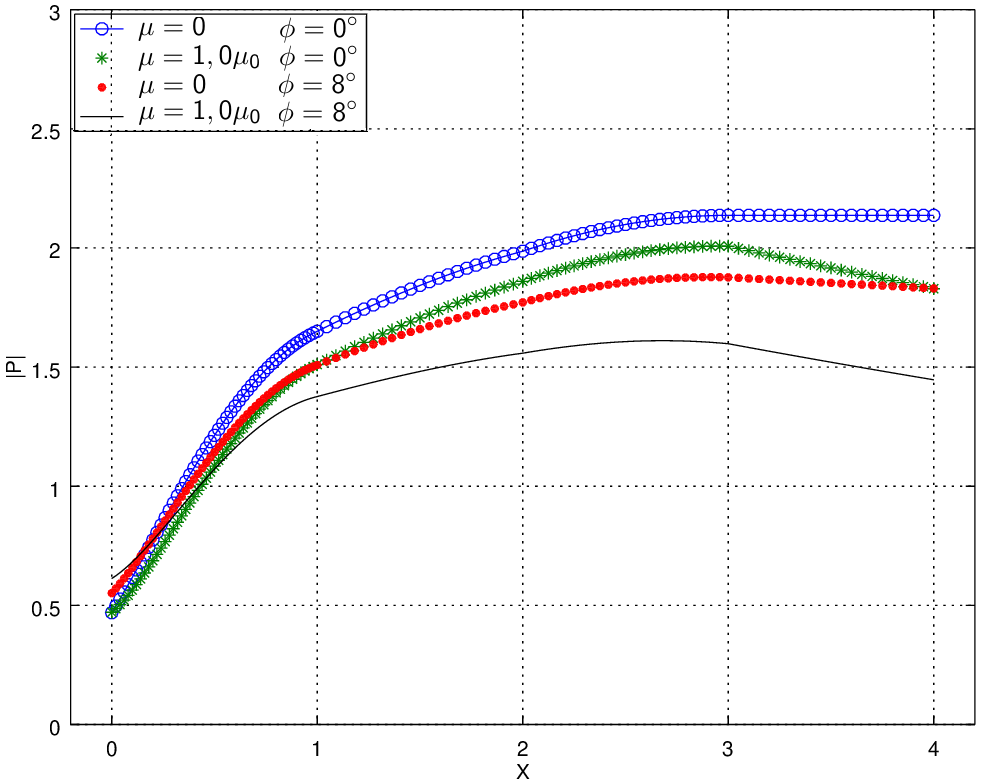
\includegraphics[scale=0.7]{Figures/fig5_P_f3_65_viscoelasticity_viscosity_NEW.png}\\
	(b)\\
	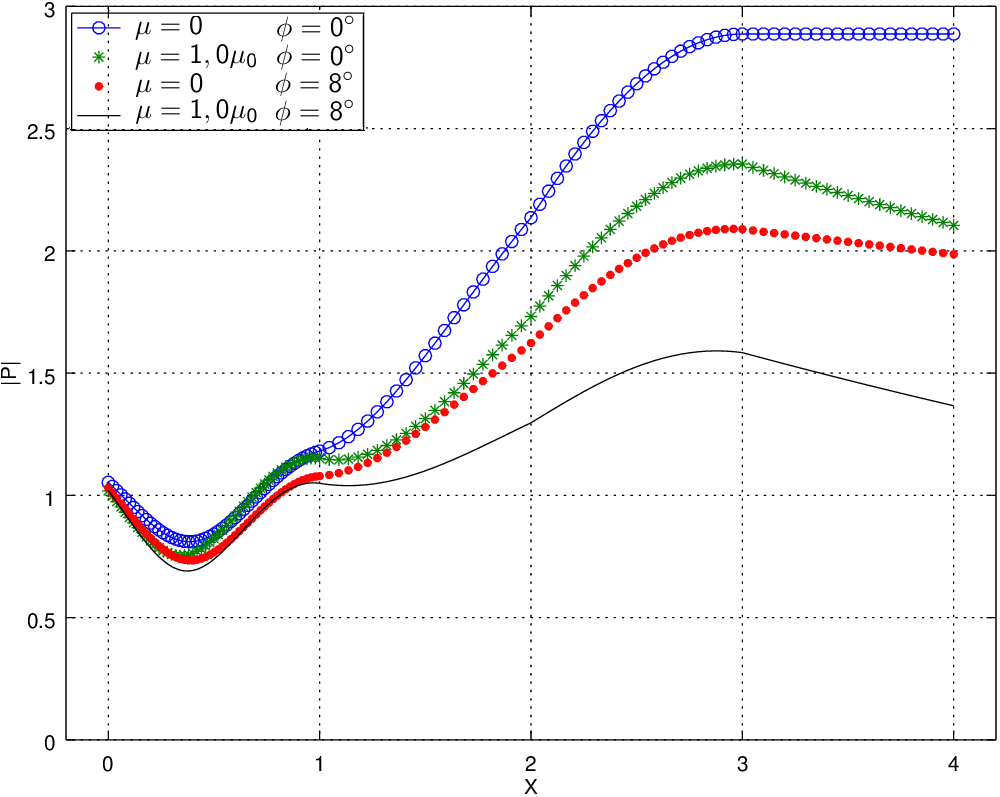
\includegraphics[scale=0.7]{Figures/fig5_P_f7_30_viscoelasticity_viscosity_NEW.png}\\
	\caption{Amplitude da pressão $|P|$ ao longo da árvore arterial considerando diferentes valores de viscoelasticidade $\phi_0$ e frequências: (a) $f$ = 3,65 Hz, (b)  $f$ = 7,30 Hz. }
	\label{fig5a:arterial-tree}%
\end{figure}

\begin{figure}[!htbp]
	\centering
	(a) $f$ = 10,95 Hz\\
	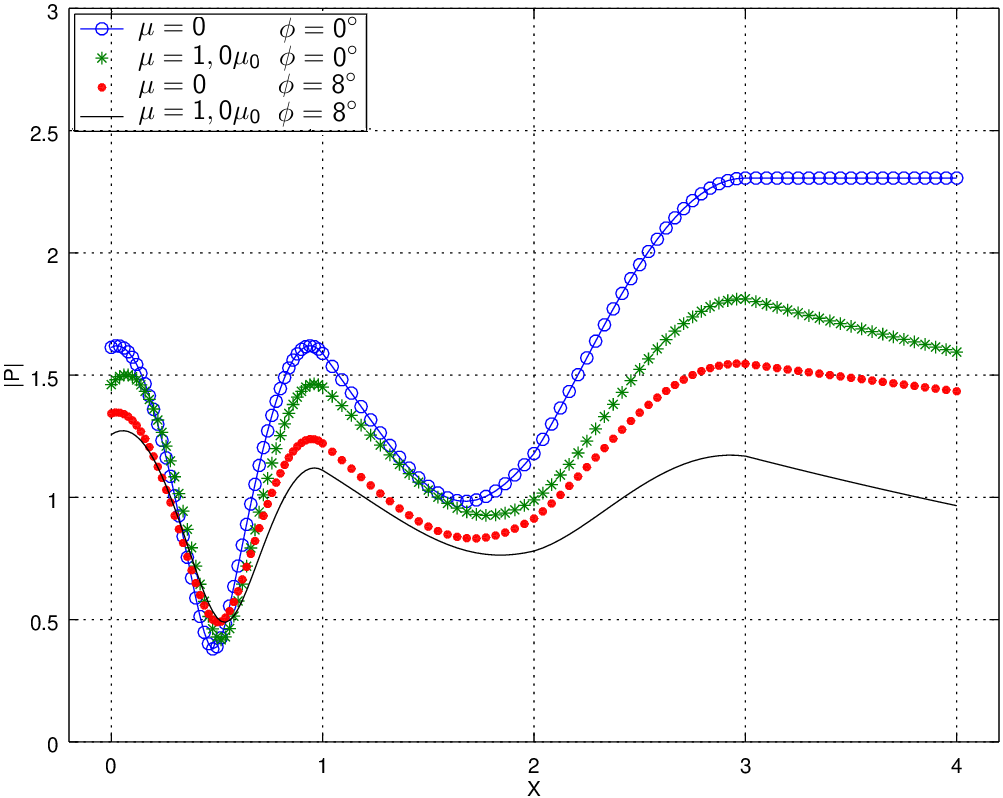
\includegraphics[scale=0.7]{Figures/fig5_P_f10_95_viscoelasticity_viscosity_NEW.png}\\
	(b) $f$ = 14,60 Hz\\
	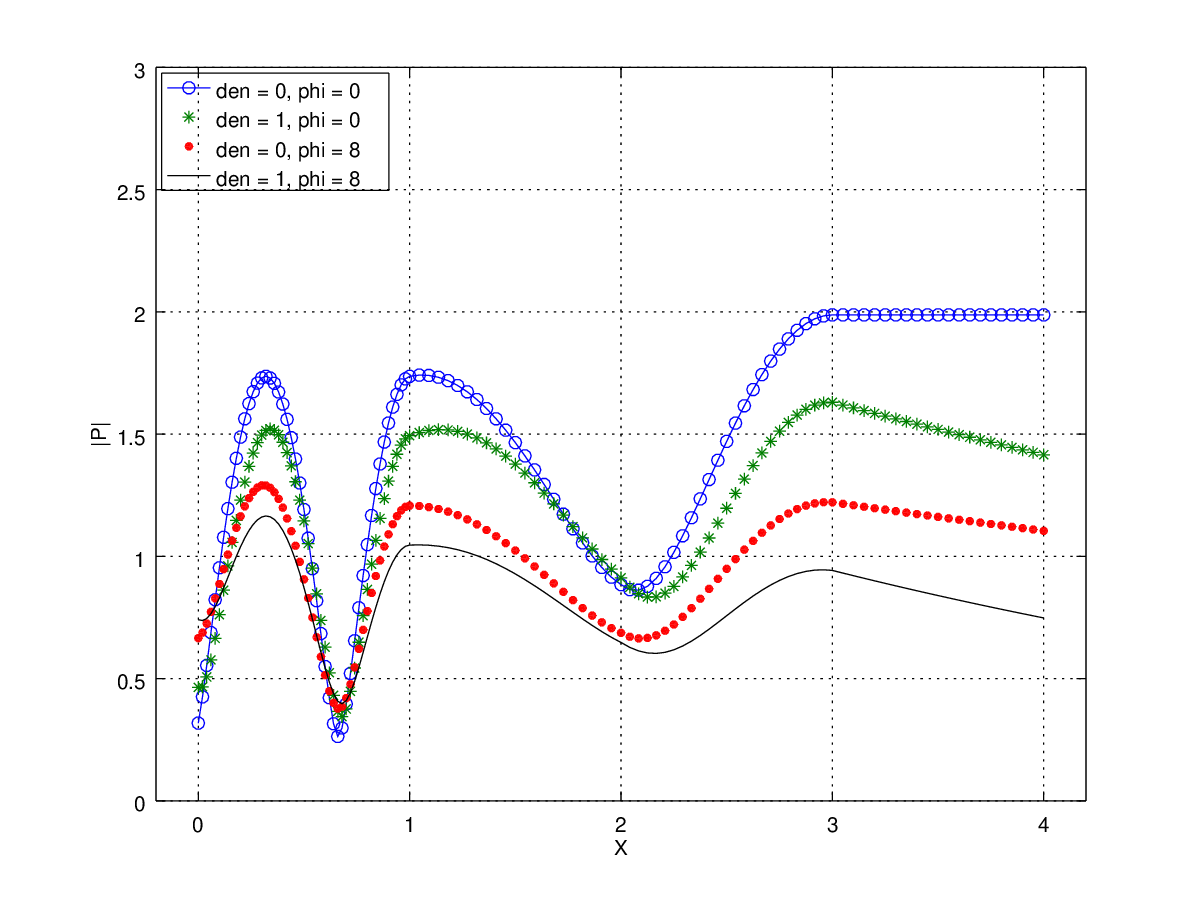
\includegraphics[scale=0.7]{Figures/fig5_P_f14_60_viscoelasticity_viscosity.png}\\
	\caption{Amplitude da pressão $|P|$ ao longo da árvore arterial considerando diferentes valores de viscoelasticidade $\phi_0$ e frequências: (a) $f$ = 10,95 Hz, (b) $f$ = 14,60 Hz.}
	\label{fig5b:arterial-tree}%
\end{figure}

%--------------------------------------------------------------------------------%
\section{ANÁLISES DE DESEMPENHO DA FERRAMENTA COMPUTACIONAL}\label{sec:resultados2}
\justifying

Nesta seção, apresentam-se resultados obtidos com a implementação da ferramenta computacional em seus dois ambientes \textit{IGU} e \textit{InGU}. As simulações realizadas aqui tratam da aplicação da ferramenta na obtenção de resultados do escoamento pulsátil em um modelo de árvore arterial. Os resultados de ambas as versões serão apresentados e comparados com a versão anteriormente apresentada.

Na Figura~\ref{fig:cmake}, tem-se selecionado o arquivo \textit{CMakeLists.txt} é o responsável por interpretar o projeto \textit{Qt} e corretamente compilar as bibliotecas necessárias. Na interface \textit{IDE} do \textit{QtCreator}, este arquivo contém as instruções para compilar todos os ambientes deste trabalho e um ambiente com a versão \textit{alpha} da ferramenta computacional \textit{IGU0}. A versão \textit{alpha} da ferramenta computacional \textit{IGU} exporta seus resultados em arquivos \textit{VTK}, que podem ser lidos pela nova versão da ferramenta ou ainda utilizados em outro ambiente.


\begin{figure}[!htbp]
	\centering
	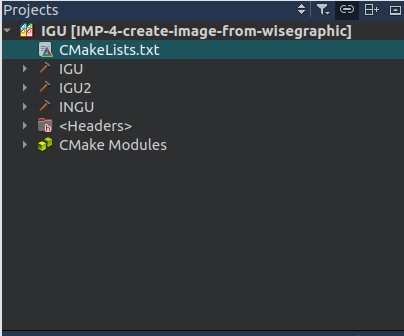
\includegraphics[scale=1.5]{Figures/cmake_print.png}
	\caption{Representação do projeto aberto através do arquivo \textit{CMakeLists.txt} na interface \textit{IDE} do \textit{QtCreator}.}
	\label{fig:cmake}
\end{figure}


Ao abrir o arquivo do projeto é possível verificar a existência de três projetos à serem compilados: (1) \textit{IGU0}, contendo a versão \textit{alpha} do programa com interface; (2) \textit{IGU}, que é a versão atual da ferramenta com interface gráfica apresentada neste trabalho; e (3) \textit{InGU} que é a versão atual da ferramenta sem uma interface gráfica. Podemos ver estes projetos presentes na Figura~\ref{fig:cmake}.

Ao executar a versão \textit{alpha}, ferramenta computacional uma estrutura de dados sem o conceito de Fábricas e classes de propósito único é utilizada no processo de compilação. Por outro lado, os ambientes \textit{IGU} e \textit{InGU} utilizam as mesmas classes e a mesma estrutura de dados.


\begin{figure}[!htbp]
	\centering
	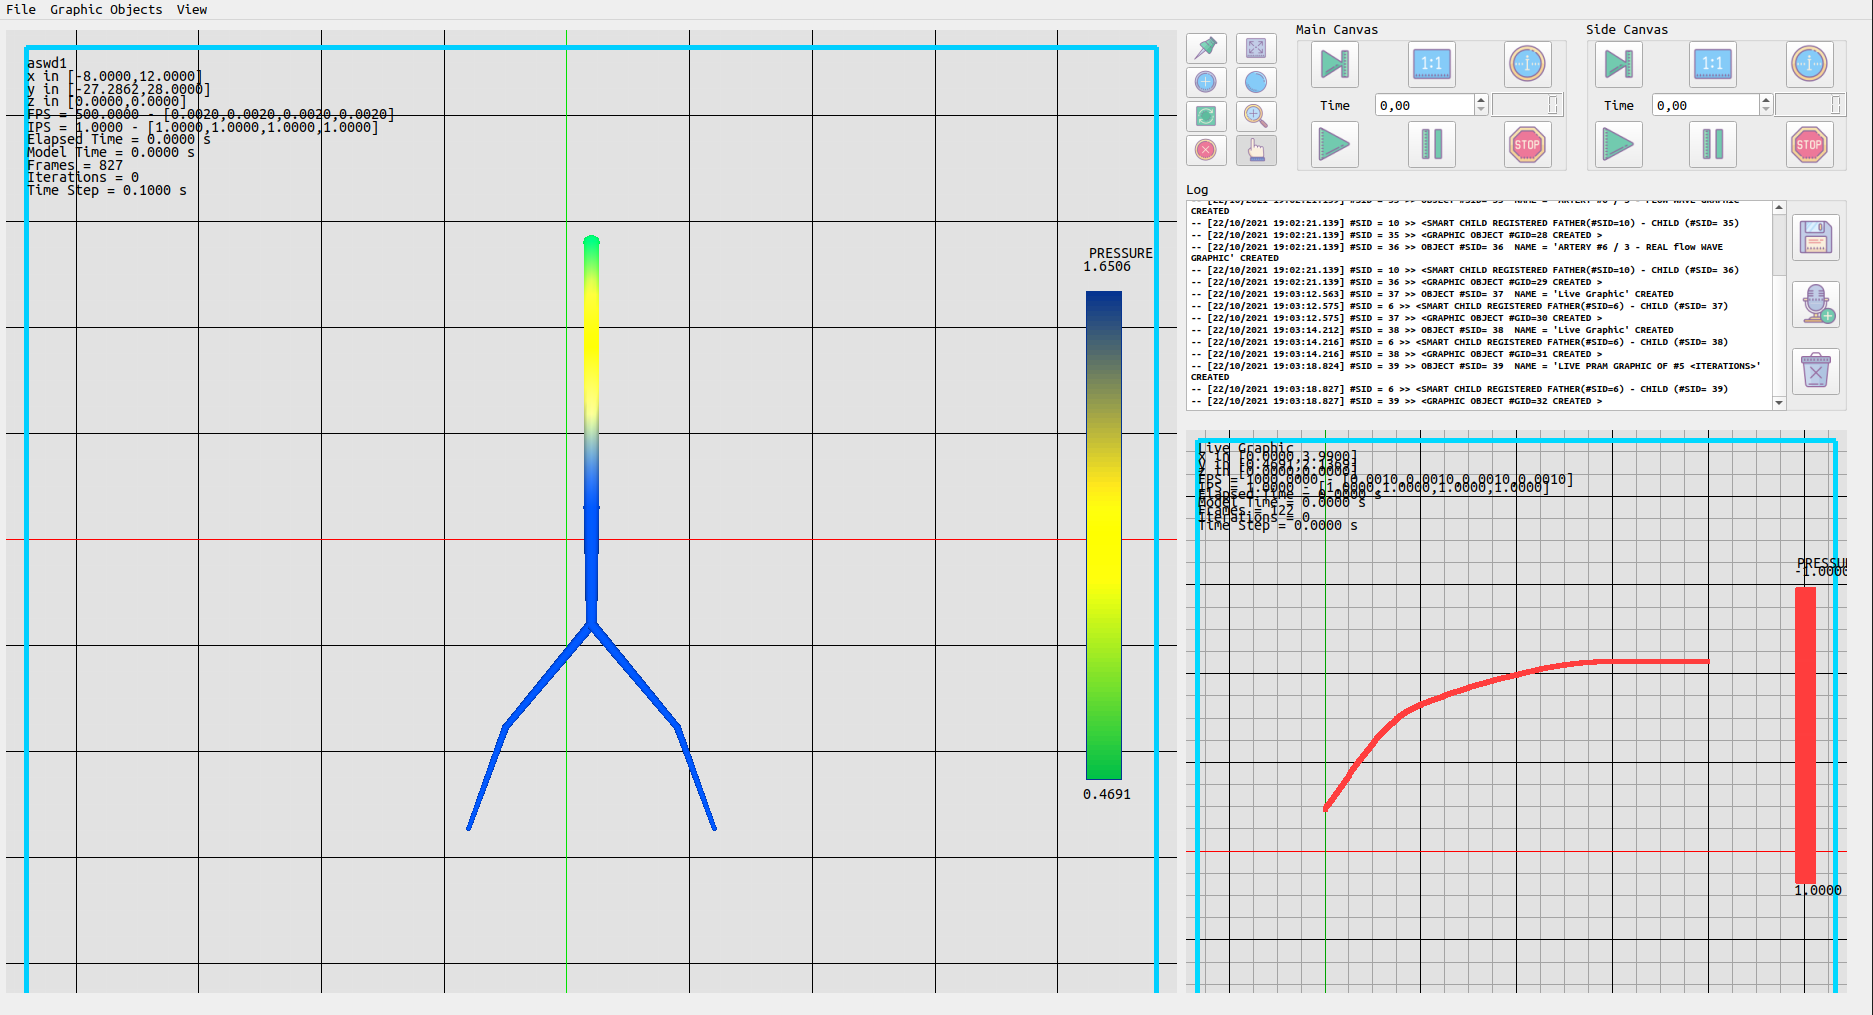
\includegraphics[width=\linewidth]{Figures/IGU_old2.png}
	\caption{Ferramenta computacional \textit{IGU0}.}
	\label{fig:IGU-old}
\end{figure}

Na Figura~\ref{fig:IGU-old} pode ser observado que a interface gráfica do usuário possui duas telas de \textit{Canvas} e diversos botões na janela principal. O funcionamento desta interface é muito similar ao da nova interface, entretanto está muito mais ligada exclusivamente à simulação do escoamento pulsátil. Dois \textit{Canvas} possibilitam a exibição de uma árvore arterial e seu gráfico ao mesmo tempo com a propriedade hemodinâmica calculada (no exemplo, a pressão ao longo dos vasos), entretanto fixa estes dois elementos na janela principal. Com o esquema de janelas desenvolvido no ambiente \textit{IGU} é possível que diversos objetos gráficos sejam exibidos ao mesmo tempo e estas janelas escaladas independentemente.

A estrutura de dados do ambiente \textit{IGU0} não apresenta os conceitos de fábrica e é incapaz de armazenar todos os estados do modelo geométrico. Logo, caso se deseje recuperar um estado anterior é necessário reiniciar o experimento.

No ambiente \textit{IGU0}, o processo iterativo dos modelos estava atrelada ao uso da interface de usuário, sem a possibilidade de executar uma sequência de comandos de uma só vez. Portanto, não é possível mensurar claramente o tempo de execução de um trabalho no ambiente \textit{IGU0}, porque o seu processo de configuração requer interação com a interface de usuário. Através dos comandos disponibilizados na Seção~\ref{sec:console}, presentes nos ambientes \textit{IGU} e \textit{InGU}, é possível que objetos inteligentes executem uma bateria de comandos e tenha seu desempenho mensurado e analisado.

Finalmente, como visto na Seção~\ref{sec:threads}, a ferramenta (\textit{IGU} e \textit{InGU}) utiliza a \textit{thread} \textit{WiseProcessor} para processar o objeto \textit{WiseObject}. Este recurso permite que ferramenta execute o ciclo de iteração sem afetas o funcionamento da interface gráfica de usuário ou bloquear seus processos e funcionalidades.

Para quantificar o desempenho trazido da ferramenta computacional \textit{INGU}, um experimento foi realizado. Este experimento consistiu no cálculo da distribuição da amplitude de pressão ao longo da árvore arterial (ver Figura~\ref{fig:arvore-canina}) considerando diferentes parâmetros: (i) viscosidade $\mu$, (ii) ângulo de faze $\phi$ e (iii) frequência $f$. Em suma, os três cenários da Seção~\ref{sec:resultados} são aqui contemplados.

\begin{table}[!htbp]
	\caption{Parâmetros de entrada utilizados no teste de carga.}
	\centering{}
	\begin{tabular}{c|c}
		\toprule 
		Frequência	& $f \in \{3,65;7,30;10,95;14,60\}$  \\
		\midrule 
		Viscosidade	& $\mu \in \{0;0,5\mu_0;1,0\mu_0;1,5\mu_0\}$    \\ 
		\midrule 
		Ângulo de Fase	& $\phi_0 \in \{0{\circ},4{\circ},8{\circ},12{\circ}\}$  \\ 
		\bottomrule 
	\end{tabular} 
	\label{tab1:entrada}
\end{table}

Na Tabela~\ref{tab1:entrada}, apresentam-se os parâmetros de entrada utilizados para testar o desempenho da ferramenta \textit{InGU}. O objetivo é realizar $64$ iterações combinando os parâmetros de entrada e armazenar o tempo de execução. Cada iteração irá executar o experimento com uma combinação dos três parâmetros de entrada.

O gerenciador de \textit{threads} \textit{WiseThreadPool} é o responsável por gerenciar a quantidade de \textit{threads} utilizada pela ferramenta. Primeiramente, observou-se que a simulação do modelo matemático para um determinado conjunto de parâmetros possui escolhido possui uma média tempo de execução de $30ms$, enquanto uma operação de escrita e leitura demora entre$100$ e $300ms$. Como o ciclo de iteração de um objeto \textit{WiseObject} envolve diretamente operações de escrita e leitura, estas foram as \textit{threads} escolhidas à serem duplicadas. \textit{Threads} do tipo \textit{WiseConsole} e \textit{WiseProcessor} requerem uma quantidade maior de trabalhos para que se obtenha algum aumento de desempenho, no experimento escolhido o aumento da quantidade destas \textit{threads} implica diretamente no aumento do tempo de execução devido à comunicação entre as \textit{threads}.

O experimento foi executado em uma máquina com o processador \textit{Intel Core I9-9900K@3.60GHz} com $4GB@2300MHz$ de memória RAM disponíveis. Para medir o tempo de execução o ambiente computacional \textit{InGU}, por não possuir interface gráfica demonstrou ser o mais rápido durante os testes.


\begin{figure}[!htbp]
	\centering
	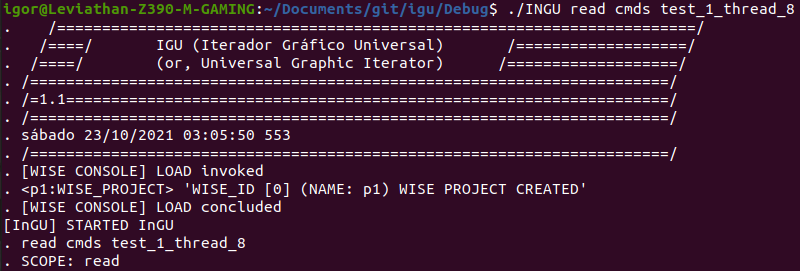
\includegraphics[width=\linewidth]{Figures/INGU.png}
	\caption{Ferramenta computacional \textit{InGU} executando o comando de leitura de arquivo de entrada.}
	\label{fig:INGU}
\end{figure}

Para executar o teste um arquivo de entrada com uma lista de comandos, assim como o Anexo~\ref{annex2}, foi confeccionado para criar a estrutura, realizar os cálculos, salvar os resultados e limpar o ambiente. O ambiente computacional \textit{InGU} permite sua execução com parâmetros de entrada. Ao executar o comando "\textit{./INGU read cmds arquivo}" o ambiente computacional executa o comando de leitura de arquivo de entrada e finaliza o programa. A Figura~\ref{fig:INGU} mostra este comportamento.

Para que as \textit{threads} aumentem o desempenho, os comando precisam ser divididos em cargas de trabalho. Os comandos recebidos pela ferramenta são executados de forma sequencial dentro de seus respectivos grupos de trabalho. Utilizando objetos inteligente \textit{WiseObject} distintos, grupos de trabalho diferentes podem ser executados simultaneamente. Com isto o experimento foi dividido em $4$ grupos, com o número de grupo de trabalhos $w \in {1,2,4,8}$ ob tendo o tempo de execução para o número de \textit{threads} $t \in {1,2,4,8}$. Como as cargas de trabalho não compartilham objetos inteligentes \textit{WiseObject}, o uso de mais cargas afeta diretamente a quantidade de memória utilizada pela ferramenta computacional.


%--------------------------------------------------------------------------------%
\subsection{DESEMPENHO DE THREADS}\label{sec:cenario4}

Na Tabela~\ref{tab1:medium} estão registrados os tempos médios de execução do experimento.

\begin{table}[!htbp]
	\caption{Tempo de execução média em milissegundos $ms$ do ciclo de iteração com diferentes arranjos de \textit{threads}, em negrito os melhores tempos.}
	\centering{}
	\begin{tabular}{c|c|c|c|c}
		\toprule 
		\textbf{Cargas de Trabalho}	& $1$ & $2$ & $4$  & $8$\\ 
		\midrule 
		\textbf{1 Thread} & 7854,4 &	4475,4 &	2810,6 &	2453,6\\ 
		\midrule 
		\textbf{2 Threads} & \textbf{5078,8} &	\textbf{3543,6} &	2885,8 &	2564,4\\ 
		\midrule 
		\textbf{4 Threads} & 5232,4 &	3286 &	\textbf{2239,8} &	\textbf{1959,6}\\ 
		\midrule 
		\textbf{8 Threads} & 7677 &	4545,4 &	2887,8 &	2452,6
		
		\\ 
		\bottomrule 
	\end{tabular} 
	\label{tab1:medium}
\end{table}

Com estes tempos de execução construiu-se Tabela~\ref{tab1:speedup} contendo o cálculo do ganho de performance ao duplicar o número de \textit{threads}. O \textit{speed up} $S_th$ caculado nesta tabela quantifica é dado por:

\begin{equation}
	S_th = t_{th-1}/t_{th},
	\label{eq:speedup1}
\end{equation}
sendo $th \in \{1,2,4,8\}$ a quantidade de \textit{threads}.

\begin{table}[!htbp]
\caption{\textit{Speed up} do ciclo de iteração com diferentes arranjos de \textit{threads}, em negrito os melhores aumentos de desempenho.}
\centering{}
\begin{tabular}{c|c|c|c|c}
	\toprule 
	\textbf{Cargas de Trabalho}	& $1$ & $2$ & $4$  & $8$\\ 
	\midrule 
	\textbf{2 Threads} & \textbf{1,54650} &	\textbf{1,26295} & 0,97394 &	0,95679\\ 
	\midrule 
	\textbf{4 Threads} & 0,970641 &	1,07839 &	\textbf{1,28841} & \textbf{1,30863}\\ 
	\midrule 
	\textbf{8 Threads} & 0,68156 &	0,72292 & 0,77560 & 0,79898
	\\ 
	\bottomrule 
\end{tabular} 
\label{tab1:speedup}
\end{table}

Ao duplicar o número de \textit{threads} é esperado um \textit{speed up} de $2$, entretanto a comunicação entre as \textit{threads} não permite que este número seja alcançado; Após uma quantidade de \textit{threads} este número passa a cair com a adição de novas \textit{threads}. Observamos que no caso da ferramenta computacional, reorganizar o experimento em cargas de trabalho é capaz de aumentar a velocidade da execução até mesmo em sistema com apenas uma \textit{thread}.

Os resultados obtidos com $2$ e $4$ \textit{threads} foram os melhores, com esta quantidade de \textit{threads} e com o aumento da quantidade de cargas de trabalho é possível melhorar drasticamente o desempenho da ferramenta. Com $8$ \textit{threads} a ferramenta computacional apresenta um tempo médio de execução mesmo com uma quantidade maior de trabalhos.

%--------------------------------------------------------------------------------%
\subsection{DESEMPENHO DE CARGA DE TRABALHO}\label{sec:cenario5}

Com os mesmos resultados de tempo apresentados na Tabela~\ref{tab1:medium} foi calculado a melhora de desempenho pela utilização de uma quantidade maior de cargas de trabalho $w$. O \textit{speed up} $S_w$ caculado nesta tabela quantifica é dado por:

\begin{equation}
	S_w = t_{w-1}/t_{w},
	\label{eq:speedup2}
\end{equation}
sendo $w \in \{1,2,4,8\}$ a quantidade cargas de trabalho.

\begin{table}[!htbp]
\caption{\textit{Speed up} do ciclo de iteração com diferentes arranjos de cargas de trabalho $w$, em negrito os melhores aumentos de desempenho.}
\centering{}
\begin{tabular}{c|c|c|c}
	\toprule 
	\textbf{Cargas de Trabalho} & $2$ & $4$  & $8$\\ 
	\midrule 
	\textbf{1 Thread} & \textbf{1,755} &	\textbf{1,5923} &	\textbf{1,1455} \\ 
	\midrule 
	\textbf{2 Threads} & 1,4332 &	1,2279 & 1,1253\\ 
	\midrule 
	\textbf{4 Threads} & 1,5923 &	1,4671 &	1,143\\ 
	\midrule 
	\textbf{8 Threads} & 1,689 &	1,574 & 1,1774	\\ 
	\bottomrule 
\end{tabular} 
\label{tab1:speedup2}
\end{table}

Ao duplicar o número de cargas de trabalho $w$ é observada uma melhora expressiva no ambiente executado com uma \textit{thread}, mostrando que a ferramenta é capaz de tirar proveito dos recursos da máquina mesmo que não hajam diversos núcleos de processamento disponíveis. Diferentemente do \textit{speed up} calculado no aumento de \textit{threads}, neste caso há sempre uma melhora de desempenho.